\documentclass[ignorenonframetext,]{beamer}
\setbeamertemplate{caption}[numbered]
\setbeamertemplate{caption label separator}{: }
\setbeamercolor{caption name}{fg=normal text.fg}
\beamertemplatenavigationsymbolsempty
\usepackage{lmodern}
\usepackage{amssymb,amsmath}
\usepackage{ifxetex,ifluatex}
\usepackage{fixltx2e} % provides \textsubscript
\ifnum 0\ifxetex 1\fi\ifluatex 1\fi=0 % if pdftex
\usepackage[T1]{fontenc}
\usepackage[utf8]{inputenc}
\else % if luatex or xelatex
\ifxetex
\usepackage{mathspec}
\else
\usepackage{fontspec}
\fi
\defaultfontfeatures{Ligatures=TeX,Scale=MatchLowercase}
\fi
\usetheme{metropolis}
% use upquote if available, for straight quotes in verbatim environments
\IfFileExists{upquote.sty}{\usepackage{upquote}}{}
% use microtype if available
\IfFileExists{microtype.sty}{%
\usepackage{microtype}
\UseMicrotypeSet[protrusion]{basicmath} % disable protrusion for tt fonts
}{}
\newif\ifbibliography
\usepackage{color}
\usepackage{fancyvrb}
\newcommand{\VerbBar}{|}
\newcommand{\VERB}{\Verb[commandchars=\\\{\}]}
\DefineVerbatimEnvironment{Highlighting}{Verbatim}{commandchars=\\\{\}}
% Add ',fontsize=\small' for more characters per line
\usepackage{framed}
\definecolor{shadecolor}{RGB}{248,248,248}
\newenvironment{Shaded}{\begin{snugshade}}{\end{snugshade}}
\newcommand{\KeywordTok}[1]{\textcolor[rgb]{0.13,0.29,0.53}{\textbf{{#1}}}}
\newcommand{\DataTypeTok}[1]{\textcolor[rgb]{0.13,0.29,0.53}{{#1}}}
\newcommand{\DecValTok}[1]{\textcolor[rgb]{0.00,0.00,0.81}{{#1}}}
\newcommand{\BaseNTok}[1]{\textcolor[rgb]{0.00,0.00,0.81}{{#1}}}
\newcommand{\FloatTok}[1]{\textcolor[rgb]{0.00,0.00,0.81}{{#1}}}
\newcommand{\ConstantTok}[1]{\textcolor[rgb]{0.00,0.00,0.00}{{#1}}}
\newcommand{\CharTok}[1]{\textcolor[rgb]{0.31,0.60,0.02}{{#1}}}
\newcommand{\SpecialCharTok}[1]{\textcolor[rgb]{0.00,0.00,0.00}{{#1}}}
\newcommand{\StringTok}[1]{\textcolor[rgb]{0.31,0.60,0.02}{{#1}}}
\newcommand{\VerbatimStringTok}[1]{\textcolor[rgb]{0.31,0.60,0.02}{{#1}}}
\newcommand{\SpecialStringTok}[1]{\textcolor[rgb]{0.31,0.60,0.02}{{#1}}}
\newcommand{\ImportTok}[1]{{#1}}
\newcommand{\CommentTok}[1]{\textcolor[rgb]{0.56,0.35,0.01}{\textit{{#1}}}}
\newcommand{\DocumentationTok}[1]{\textcolor[rgb]{0.56,0.35,0.01}{\textbf{\textit{{#1}}}}}
\newcommand{\AnnotationTok}[1]{\textcolor[rgb]{0.56,0.35,0.01}{\textbf{\textit{{#1}}}}}
\newcommand{\CommentVarTok}[1]{\textcolor[rgb]{0.56,0.35,0.01}{\textbf{\textit{{#1}}}}}
\newcommand{\OtherTok}[1]{\textcolor[rgb]{0.56,0.35,0.01}{{#1}}}
\newcommand{\FunctionTok}[1]{\textcolor[rgb]{0.00,0.00,0.00}{{#1}}}
\newcommand{\VariableTok}[1]{\textcolor[rgb]{0.00,0.00,0.00}{{#1}}}
\newcommand{\ControlFlowTok}[1]{\textcolor[rgb]{0.13,0.29,0.53}{\textbf{{#1}}}}
\newcommand{\OperatorTok}[1]{\textcolor[rgb]{0.81,0.36,0.00}{\textbf{{#1}}}}
\newcommand{\BuiltInTok}[1]{{#1}}
\newcommand{\ExtensionTok}[1]{{#1}}
\newcommand{\PreprocessorTok}[1]{\textcolor[rgb]{0.56,0.35,0.01}{\textit{{#1}}}}
\newcommand{\AttributeTok}[1]{\textcolor[rgb]{0.77,0.63,0.00}{{#1}}}
\newcommand{\RegionMarkerTok}[1]{{#1}}
\newcommand{\InformationTok}[1]{\textcolor[rgb]{0.56,0.35,0.01}{\textbf{\textit{{#1}}}}}
\newcommand{\WarningTok}[1]{\textcolor[rgb]{0.56,0.35,0.01}{\textbf{\textit{{#1}}}}}
\newcommand{\AlertTok}[1]{\textcolor[rgb]{0.94,0.16,0.16}{{#1}}}
\newcommand{\ErrorTok}[1]{\textcolor[rgb]{0.64,0.00,0.00}{\textbf{{#1}}}}
\newcommand{\NormalTok}[1]{{#1}}

% Prevent slide breaks in the middle of a paragraph:
\widowpenalties 1 10000
\raggedbottom

\AtBeginPart{
\let\insertpartnumber\relax
\let\partname\relax
\frame{\partpage}
}
\AtBeginSection{
\ifbibliography
\else
\let\insertsectionnumber\relax
\let\sectionname\relax
\frame{\sectionpage}
\fi
}
\AtBeginSubsection{
\let\insertsubsectionnumber\relax
\let\subsectionname\relax
\frame{\subsectionpage}
}

\setlength{\parindent}{0pt}
\setlength{\parskip}{6pt plus 2pt minus 1pt}
\setlength{\emergencystretch}{3em}  % prevent overfull lines
\providecommand{\tightlist}{%
\setlength{\itemsep}{0pt}\setlength{\parskip}{0pt}}
\setcounter{secnumdepth}{0}

\title{Chapter 2: Manipulating Your Data}
\author{Tyson S. Barrett}
\date{Summer 2017}

\begin{document}
\frame{\titlepage}

\begin{frame}
\tableofcontents[hideallsubsections]
\end{frame}

\section{Introduction}\label{introduction}

\begin{frame}{The Newest and Brightest}

\centerline{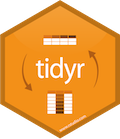
\includegraphics[height=2in]{Figures/tidyr_logo.png} \text{  \LARGE    }

\includegraphics[height=2in]{Figures/pipe_logo.png}}

\end{frame}

\begin{frame}[fragile]{The Newest and Brightest}

\begin{block}{Tidyverse}

\begin{itemize}
\tightlist
\item
  In order to manipulate your data in the cleanest, most up-to-date
  manner, we are going to be using the ``tidyverse'' group of methods.
\item
  The tidyverse\footnote<.->{Hadley Wickham (2016). tidyverse: Easily
    Install and Load `Tidyverse' Packages. R package version 1.0.0.
    \url{https://CRAN.R-project.org/package=tidyverse}} is a group of
  packages\footnote<.->{Remember, a package is an extension to
    \texttt{R} that gives you more functions that you can easily load
    into \texttt{R}.} that provide a simple syntax that can do many
  basic (and complex) data manipulating.
\item
  The group of packages can be downloaded via:
\end{itemize}

\begin{Shaded}
\begin{Highlighting}[]
\KeywordTok{install.packages}\NormalTok{(}\StringTok{"tidyverse"}\NormalTok{)}
\end{Highlighting}
\end{Shaded}

After downloading it, simply use:

\begin{Shaded}
\begin{Highlighting}[]
\KeywordTok{library}\NormalTok{(tidyverse)}
\end{Highlighting}
\end{Shaded}

\begin{verbatim}
Loading tidyverse: ggplot2
Loading tidyverse: tibble
Loading tidyverse: tidyr
Loading tidyverse: readr
Loading tidyverse: purrr
Loading tidyverse: dplyr
\end{verbatim}

\begin{verbatim}
Conflicts with tidy packages ----------------------------------------------
\end{verbatim}

\begin{verbatim}
filter(): dplyr, stats
lag():    dplyr, stats
\end{verbatim}

\end{block}

\end{frame}

\begin{frame}[fragile]{Tidyverse}

Note that when we loaded tidyverse it loaded 6 packages and told you of
``conflicts''. These conflicts are where two or more loaded packages
have the same function in them. The last loaded package is the one that
\texttt{R} will use by default. For example, if we loaded two
packages--\texttt{awesome} and \texttt{amazing}--and both had the
function--\texttt{make\_really\_great} and we loaded \texttt{awesome}
and then \texttt{amazing} as so:

\begin{Shaded}
\begin{Highlighting}[]
\KeywordTok{library}\NormalTok{(awesome)}
\KeywordTok{library}\NormalTok{(amazing)}
\end{Highlighting}
\end{Shaded}

\texttt{R} will automatically use the function from \texttt{amazing}.

\end{frame}

\begin{frame}[fragile]{Conflicts}

We can still access the \texttt{awesome} version of the function
(because even though the name is the same, they won't necessarily do the
same things for you). We can do this by:

\begin{Shaded}
\begin{Highlighting}[]
\NormalTok{awesome::}\KeywordTok{make_really_great}\NormalTok{(arg)}
\end{Highlighting}
\end{Shaded}

That's a bit of an aside, but know that you can always get at a function
even if it is ``masked'' from your current session.

\end{frame}

\section{Tidy Methods}\label{tidy-methods}

\begin{frame}[fragile]{The Tidy Data Way}

I'm introducing this to you for a couple reasons.

\begin{enumerate}
\def\labelenumi{\arabic{enumi}.}
\tightlist
\item
  It simplifies the code and makes the code more readable. As
  Mr.~Wickham says, \textbf{there are always at least two collaborators
  on any project: you and future you.}
\item
  It is the cutting edge. The most influential individuals in the
  \texttt{R} world, including the makers and maintainers of
  \texttt{RStudio}, use these methods and syntax.
\end{enumerate}

The majority of what you'll need to do with data as a researcher will be
covered by these functions.

\end{frame}

\begin{frame}{Methods for Tidying}

There are several methods that help tidy up your data:

\begin{enumerate}
\def\labelenumi{\arabic{enumi}.}
\tightlist
\item
  Piping
\item
  Selecting and Filtering
\item
  Grouping and Summarizing
\item
  Reshaping
\item
  Joining (merging)
\end{enumerate}

To help illustrate each aspect, we are going to use real data from the
National Health and Nutrition Examiniation Survey (NHANES). I've
provided this data at
\url{https://tysonstanley.github.io/assets/Data/NHANES.zip}. I've
cleaned it up somewhat already.

\end{frame}

\section{Example}\label{example}

\begin{frame}[fragile]{Example: NHANES}

\begin{block}{Import}

First, we will set our working directory with \texttt{setwd}. This tells
\texttt{R} where to look for files, including your data files.

\begin{Shaded}
\begin{Highlighting}[]
\KeywordTok{setwd}\NormalTok{(}\StringTok{"~/Dropbox/GitHub/blog_rstats/assets/Data/"}\NormalTok{)}
\end{Highlighting}
\end{Shaded}

\begin{Shaded}
\begin{Highlighting}[]
\KeywordTok{library}\NormalTok{(foreign)}
\NormalTok{dem_df <-}\StringTok{ }\KeywordTok{read.xport}\NormalTok{(}\StringTok{"NHANES_demographics_11.xpt"}\NormalTok{)}
\NormalTok{med_df <-}\StringTok{ }\KeywordTok{read.xport}\NormalTok{(}\StringTok{"NHANES_MedHeath_11.xpt"}\NormalTok{)}
\NormalTok{men_df <-}\StringTok{ }\KeywordTok{read.xport}\NormalTok{(}\StringTok{"NHANES_MentHealth_11.xpt"}\NormalTok{)}
\NormalTok{act_df <-}\StringTok{ }\KeywordTok{read.xport}\NormalTok{(}\StringTok{"NHANES_PhysActivity_11.xpt"}\NormalTok{)}
\end{Highlighting}
\end{Shaded}

\end{block}

\end{frame}

\begin{frame}[fragile]{Example: NHANES}

Now we have four separate, but related, data sets in memory:

\begin{enumerate}
\def\labelenumi{\arabic{enumi}.}
\tightlist
\item
  \texttt{dem\_df} containing demographic information
\item
  \texttt{med\_df} containing medical health information
\item
  \texttt{men\_df} containing mental health information
\item
  \texttt{act\_df} containing activity level information
\end{enumerate}

\end{frame}

\begin{frame}[fragile]{Example: NHANES}

Since all of them have all-cap variable names, we are going to quickly
change this with a little trick:

\begin{Shaded}
\begin{Highlighting}[]
\KeywordTok{names}\NormalTok{(dem_df) <-}\StringTok{ }\KeywordTok{tolower}\NormalTok{(}\KeywordTok{names}\NormalTok{(dem_df))}
\KeywordTok{names}\NormalTok{(med_df) <-}\StringTok{ }\KeywordTok{tolower}\NormalTok{(}\KeywordTok{names}\NormalTok{(med_df))}
\KeywordTok{names}\NormalTok{(men_df) <-}\StringTok{ }\KeywordTok{tolower}\NormalTok{(}\KeywordTok{names}\NormalTok{(men_df))}
\KeywordTok{names}\NormalTok{(act_df) <-}\StringTok{ }\KeywordTok{tolower}\NormalTok{(}\KeywordTok{names}\NormalTok{(act_df))}
\end{Highlighting}
\end{Shaded}

This takes the names of the data frame (on the right hand side), changes
them to lower case and then reassigns them to the names of the data
frame.\footnote<.->{Note that these are not particularly helpful names,
  but they are the names provided in the original data source. If you
  have questions about the data, visit
  \url{http://wwwn.cdc.gov/Nchs/Nhanes/Search/Nhanes11_12.aspx}.}

\end{frame}

\begin{frame}{Example: NHANES}

\begin{block}{We will now go through each aspect of the tidy way of
working with data using these four data sets.}

\end{block}

\end{frame}

\begin{frame}{Example: NHANES}

\begin{block}{Piping}

\centering  
\includegraphics[height=2in]{Figures/pipe_logo.png}

\end{block}

\end{frame}

\begin{frame}[fragile]{Example: NHANES}

\begin{block}{Piping}

\texttt{\%\textgreater{}\%} is the pipe ``operator''. It takes what is
on the left hand side and puts it in the right hand side's function.

\begin{Shaded}
\begin{Highlighting}[]
\NormalTok{dem_df %>%}\StringTok{ }\NormalTok{summary}
\end{Highlighting}
\end{Shaded}

So the above code takes the data frame \texttt{df} and puts it into the
\texttt{summary} function. This does the same thing as
\texttt{summary(dem\_df)}.

In this simple case, it doesn't really make the code more readable, but
in more complex situations it can really help.

\end{block}

\end{frame}

\begin{frame}{Example: NHANES}

\begin{block}{Select and Filter}

\centering  
\includegraphics[height=2in]{Figures/dplyr_logo.png}

\end{block}

\end{frame}

\begin{frame}{Example: NHANES}

\begin{block}{Select and Filter}

In situations where you want or need to subset your data, two main forms
exist:

\begin{enumerate}
\def\labelenumi{\arabic{enumi}.}
\tightlist
\item
  Selecting Variables
\item
  Filtering Rows
\end{enumerate}

The following slides show the base R way and the tidyverse way of
subsetting.

\end{block}

\end{frame}

\begin{frame}[fragile]{Example: NHANES}

\textbf{Selecting Variables}

\begin{Shaded}
\begin{Highlighting}[]
\NormalTok{df[, }\KeywordTok{c}\NormalTok{(}\StringTok{"var1"}\NormalTok{, }\StringTok{"var2"}\NormalTok{, etc.)]}
\NormalTok{df %>%}
\StringTok{  }\KeywordTok{select}\NormalTok{(var1, var2, etc.)}
\end{Highlighting}
\end{Shaded}

Here both do the same thing. The first, using \texttt{{[}}, is the
``base R'' way of selecting variables. The second, using the pipe, is
the tidyverse way. Both work great so the choice is yours.

\end{frame}

\begin{frame}[fragile]{Example: NHANES}

\textbf{Filtering Rows}

\begin{Shaded}
\begin{Highlighting}[]
\NormalTok{df[df$var1 ==}\StringTok{ }\DecValTok{1}\NormalTok{, ]}
\NormalTok{df %>%}
\StringTok{  }\KeywordTok{filter}\NormalTok{(var1 ==}\StringTok{ }\DecValTok{1}\NormalTok{)}
\end{Highlighting}
\end{Shaded}

Again, both do the same thing. The first, using \texttt{{[}}, is the
``base R'' way of filtering rows so that you only keep the ones where
``var1'' in \texttt{df} is equal to \texttt{1}. Again, the second is the
tidyverse way. Whichever you like you should use.

\end{frame}

\begin{frame}[fragile]{Example: NHANES}

\begin{block}{Grouping and Summarizing}

A major aspect of analysis is comparing groups. Lucky for us, this is
very simple in \texttt{R}. I call it the three step summary:

\begin{enumerate}
\def\labelenumi{\arabic{enumi}.}
\tightlist
\item
  Data
\item
  Group by
\item
  Summarize
\end{enumerate}

\end{block}

\end{frame}

\begin{frame}[fragile]{Example: NHANES}

\begin{block}{Grouping and Summarizing}

\begin{Shaded}
\begin{Highlighting}[]
\NormalTok{dem_df$citizen <-}\StringTok{ }\KeywordTok{factor}\NormalTok{(dem_df$dmdcitzn)}
\NormalTok{dem_df %>%}\StringTok{                           }\NormalTok{## 1. Data}
\StringTok{  }\KeywordTok{group_by}\NormalTok{(citizen) %>%}\StringTok{              }\NormalTok{## 2. Group by}
\StringTok{  }\KeywordTok{summarize}\NormalTok{(}\DataTypeTok{N =} \KeywordTok{n}\NormalTok{())                 ## 3. Summarize}
\end{Highlighting}
\end{Shaded}

\begin{verbatim}
# A tibble: 4 × 2
  citizen     N
   <fctr> <int>
1       1  8685
2       2  1040
3       7    26
4      NA     5
\end{verbatim}

\end{block}

\end{frame}

\begin{frame}[fragile]{Example: NHANES}

\begin{block}{Grouping and Summarizing}

On the previous slide:

\begin{itemize}
\tightlist
\item
  The first column is the grouping variable and the second is the N
  (number of individuals) by group.
\item
  We can quickly see that there are four levels, currently, to the
  citizen variable.

  \begin{itemize}
  \tightlist
  \item
    After some reading of the documentation we see that
    \texttt{1\ =\ Citizen} and \texttt{2\ =\ Not\ a\ Citizen}.
  \item
    A value of \texttt{7} it turns out is a placeholder value for
    missing.
  \item
    And finally we have an NA category.

    \begin{itemize}
    \tightlist
    \item
      It's unlikely that we want those to be included in any analyses,
      unless we are particularly interested in the missingness on this
      variable.
    \item
      So let's do some simple cleaning to get this where we want it. To
      do this, we will use the \texttt{furniture} package.
    \end{itemize}
  \end{itemize}
\end{itemize}

\end{block}

\end{frame}

\begin{frame}[fragile]{Example: NHANES}

\begin{block}{Grouping and Summarizing}

\begin{Shaded}
\begin{Highlighting}[]
\KeywordTok{install.packages}\NormalTok{(}\StringTok{"furniture"}\NormalTok{)}
\end{Highlighting}
\end{Shaded}

\begin{Shaded}
\begin{Highlighting}[]
\KeywordTok{library}\NormalTok{(furniture)}
\NormalTok{## Changes all 7's to NA's}
\NormalTok{dem_df$citizen <-}\StringTok{ }\KeywordTok{washer}\NormalTok{(dem_df$citizen, }\DecValTok{7}\NormalTok{)         }
\NormalTok{## Changes all 2's to 0's}
\NormalTok{dem_df$citizen <-}\StringTok{ }\KeywordTok{washer}\NormalTok{(dem_df$citizen, }\DecValTok{2}\NormalTok{, }\DataTypeTok{value=}\DecValTok{0}\NormalTok{)}
\end{Highlighting}
\end{Shaded}

Now, our citizen variable is cleaned, with \texttt{0} meaning not a
citizen and \texttt{1} meaning citizen. Let's rerun the code from above
with the three step summary:

\end{block}

\end{frame}

\begin{frame}[fragile]{Example: NHANES}

\begin{block}{Grouping and Summarizing}

\begin{Shaded}
\begin{Highlighting}[]
\NormalTok{## Three step summary:}
\NormalTok{dem_df %>%}\StringTok{                           }\NormalTok{## 1. Data}
\StringTok{  }\KeywordTok{group_by}\NormalTok{(citizen) %>%}\StringTok{              }\NormalTok{## 2. Group by}
\StringTok{  }\KeywordTok{summarize}\NormalTok{(}\DataTypeTok{N =} \KeywordTok{n}\NormalTok{())                 ## 3. Summarize}
\end{Highlighting}
\end{Shaded}

\begin{verbatim}
# A tibble: 3 × 2
  citizen     N
    <chr> <int>
1       0  1040
2       1  8685
3    <NA>    31
\end{verbatim}

Its clear that the majority of the subjects are citizens.

\end{block}

\end{frame}

\begin{frame}[fragile]{Example: NHANES}

\begin{block}{Grouping and Summarizing}

\emph{Check multiple variables at the same time:}

\begin{Shaded}
\begin{Highlighting}[]
\NormalTok{## Three step summary:}
\NormalTok{dem_df %>%}\StringTok{                           }\NormalTok{## 1. Data}
\StringTok{  }\KeywordTok{group_by}\NormalTok{(citizen) %>%}\StringTok{              }\NormalTok{## 2. Group by}
\StringTok{  }\KeywordTok{summarize}\NormalTok{(}\DataTypeTok{N =} \KeywordTok{n}\NormalTok{(),                 ## 3. Summarize}
            \DataTypeTok{Age =} \KeywordTok{mean}\NormalTok{(ridageyr, }\DataTypeTok{na.rm=}\OtherTok{TRUE}\NormalTok{))                 }
\end{Highlighting}
\end{Shaded}

\begin{verbatim}
# A tibble: 3 × 3
  citizen     N      Age
    <chr> <int>    <dbl>
1       0  1040 37.31635
2       1  8685 30.66252
3    <NA>    31 40.35484
\end{verbatim}

\end{block}

\end{frame}

\begin{frame}[fragile]{Example: NHANES}

\begin{block}{Grouping and Summarizing}

On previous slide:

\begin{itemize}
\tightlist
\item
  The \texttt{n()} function gives us counts
\item
  The \texttt{mean()} function which, shockingly, gives us the mean.

  \begin{itemize}
  \tightlist
  \item
    Note that if there are \texttt{NA}'s in the variable, the mean (and
    most other functions like it) will give the result \texttt{NA}.
  \item
    To have \texttt{R} ignore these, we tell the \texttt{mean} function
    to remove the \texttt{NA}'s when you compute this using
    \texttt{na.rm=TRUE}.
  \end{itemize}
\end{itemize}

\end{block}

\end{frame}

\begin{frame}{Example: NHANES}

\centering
\textbf{The Grouping and Summarizing Steps}

This pattern of grouping and summarizing is something that will follow
us throughout the book.

It's a great way to get to know your data well and to make decisions on
what to do next with your data.

\end{frame}

\begin{frame}{Example: NHANES}

\begin{block}{Reshaping}

This is a big part of working with data. Unfortunately, it is also a
difficult topic to understand without much practice at it. In general,
two data formats exist:

\begin{enumerate}
\def\labelenumi{\arabic{enumi}.}
\tightlist
\item
  Wide form
\item
  Long form
\end{enumerate}

Only when the data is cross-sectional and each individual is a row does
this distinction not matter much. Otherwise, if there are multiple
measures per individual, or there are multiple individuals per cluster,
the distinction between wide and long is very important for modeling and
visualization.

\end{block}

\end{frame}

\begin{frame}[fragile]{Example: NHANES}

\begin{block}{Wide Form}

Wide form generally has one unit (i.e.~individual) per row. This
generally looks like:

\begin{verbatim}
   ID  Var_Time1 Var_Time2
1   1  0.4176037 0.9602761
2   2  0.7149929 0.5461098
3   3  0.7999565 0.9237952
4   4 -0.6939934 0.4098576
5   5 -1.4940423 0.9946778
6   6  1.9267254 0.4752230
7   7 -0.5157514 0.6510159
8   8 -1.3018363 0.9891306
9   9  0.4916932 0.6533781
10 10  0.9109289 0.9238842
\end{verbatim}

Notice that each row has a unique ID.

This format is common in the ANOVA family of analyses. These can be used
when there are set time points that the individual is measured and each
individual has the same number of time points. This is not always
reasonable, but when it is, wide format works just fine. However, when
these conditions don't hold, mixed effects modeling (i.e.~multilevel
modeling, hierarchical linear modeling) is particularly useful. In order
to do mixed effects modeling, long format is required.

\end{block}

\end{frame}

\begin{frame}[fragile]{Example: NHANES}

\begin{block}{Long Form}

In contrast, long format has the lowest nested unit as a single row.
This means that a single ID can span multiple rows, usually with a
unique time point for each row as so:

\begin{verbatim}
  ID Time       Var
1  1    1 0.2463071
2  1    2 0.5801360
3  1    3 0.8017131
4  1    4 0.2471068
5  2    1 0.5347363
6  2    2 0.6341020
7  3    1 0.4492248
8  3    2 0.3617016
9  3    3 0.5144749
\end{verbatim}

Notice that a single ID spans multiple columns and that each row has
only one time point. Here, time is nested within individuals making it
the lowest unit. Therefore, each row corresponds to a single time point.
Generally, this is the format we want for most modeling techniques and
most visualizations.

\end{block}

\end{frame}

\begin{frame}{Example: NHANES}

\begin{block}{Joining (merging)}

\emph{The final topic in the chapter is joining data sets.}

We currently have 4 data sets that have mostly the same people in them
but with different variables. One tells us about the demographics;
another gives us information on mental health. We may have questions
that ask whether a demographic characteristics is related to a mental
health factor. This means we need to merge, or join, our data
sets.\footnote<.->{Note that this is different than adding new rows but
  not new variables. Merging requires that we have at least some overlap
  of individuals in both data sets.}

\end{block}

\end{frame}

\begin{frame}[fragile]{Example: NHANES}

\begin{block}{Joining (merging)}

When we merge a data set, we combine them based on some ID variable(s).
Here, this is simple since each individual is given a unique identifier
in the variable \texttt{seqn}. Within the \texttt{dplyr} package there
are four main joining functions: \texttt{inner\_join},
\texttt{left\_join}, \texttt{right\_join} and \texttt{full\_join}. Each
join combines the data in slightly different ways.

\end{block}

\end{frame}

\begin{frame}[fragile]{Example: NHANES}

\begin{block}{Joining (merging)}

Let's first load \texttt{dplyr}:

\begin{Shaded}
\begin{Highlighting}[]
\KeywordTok{library}\NormalTok{(dplyr)}
\end{Highlighting}
\end{Shaded}

\end{block}

\end{frame}

\begin{frame}[fragile]{Example: NHANES}

\begin{block}{Joining (merging)}

\begin{block}{Inner Join}

Here, only those individuals that are in both data sets that you are
combining will remain. So if person ``A'' is in data set 1 and not in
data set 2 then he/she will not be included.

\begin{Shaded}
\begin{Highlighting}[]
\KeywordTok{inner_join}\NormalTok{(df1, df2, }\DataTypeTok{by=}\StringTok{"IDvariable"}\NormalTok{)}
\end{Highlighting}
\end{Shaded}

\end{block}

\end{block}

\end{frame}

\begin{frame}[fragile]{Example: NHANES}

\begin{block}{Joining (merging)}

\begin{block}{Left or Right Join}

This is similar to inner join but now if the individual is in data set 1
then \texttt{left\_join} will keep them even if they aren't in data set
2. \texttt{right\_join} means if they are in data set 2 then they will
be kept whether or not they are in data set 1.

\begin{Shaded}
\begin{Highlighting}[]
\KeywordTok{left_join}\NormalTok{(df1, df2, }\DataTypeTok{by=}\StringTok{"IDvariable"}\NormalTok{)   ## keeps all in df1}
\KeywordTok{right_join}\NormalTok{(df1, df2, }\DataTypeTok{by=}\StringTok{"IDvariable"}\NormalTok{)  ## keeps all in df2}
\end{Highlighting}
\end{Shaded}

\end{block}

\end{block}

\end{frame}

\begin{frame}[fragile]{Example: NHANES}

\begin{block}{Joining (merging)}

\begin{block}{Full Join}

This one simply keeps all individuals that are in either data set 1 or
data set 2.

\begin{Shaded}
\begin{Highlighting}[]
\KeywordTok{full_join}\NormalTok{(df1, df2, }\DataTypeTok{by=}\StringTok{"IDvariable"}\NormalTok{)}
\end{Highlighting}
\end{Shaded}

Each of the left, right and full joins will have missing values placed
in the variables where that individual wasn't found. For example, if
person ``A'' was not in df2, then in a full join they would have missing
values in the df1 variables.

\end{block}

\end{block}

\end{frame}

\begin{frame}[fragile]{Example: NHANES}

For our NHANES example, we will use \texttt{full\_join} to get all the
data sets together. Note that in the code below we do all the joining in
the same overall step.

\begin{Shaded}
\begin{Highlighting}[]
\NormalTok{df <-}\StringTok{ }\NormalTok{dem_df %>%}
\StringTok{  }\KeywordTok{full_join}\NormalTok{(med_df, }\DataTypeTok{by=}\StringTok{"seqn"}\NormalTok{) %>%}
\StringTok{  }\KeywordTok{full_join}\NormalTok{(men_df, }\DataTypeTok{by=}\StringTok{"seqn"}\NormalTok{) %>%}
\StringTok{  }\KeywordTok{full_join}\NormalTok{(act_df, }\DataTypeTok{by=}\StringTok{"seqn"}\NormalTok{)}
\end{Highlighting}
\end{Shaded}

So now \texttt{df} is the the joined data set of all four. We started
with \texttt{dem\_df} joined it with \texttt{med\_df} by \texttt{seqn}
then joined that joined data set with \texttt{men\_df} by \texttt{seqn},
and so on.

\end{frame}

\section{Conclusions}\label{conclusions}

\begin{frame}[fragile]{In This Chapter:}

\begin{itemize}
\tightlist
\item
  You have learned how to manipulate your data in several ways:

  \begin{itemize}
  \tightlist
  \item
    Summarizing
  \item
    Reshaping
  \item
    Joining
  \end{itemize}
\end{itemize}

\emph{For analyses in the next chapter, we will use this new}
\texttt{df} \emph{object that we concluded with.}

Also, you'll see that many of these methods apply to more than just
manipulating data. As you learn one method, you'll begin to see how
easily you can use it in other situations.

\end{frame}

\begin{frame}

\centerline{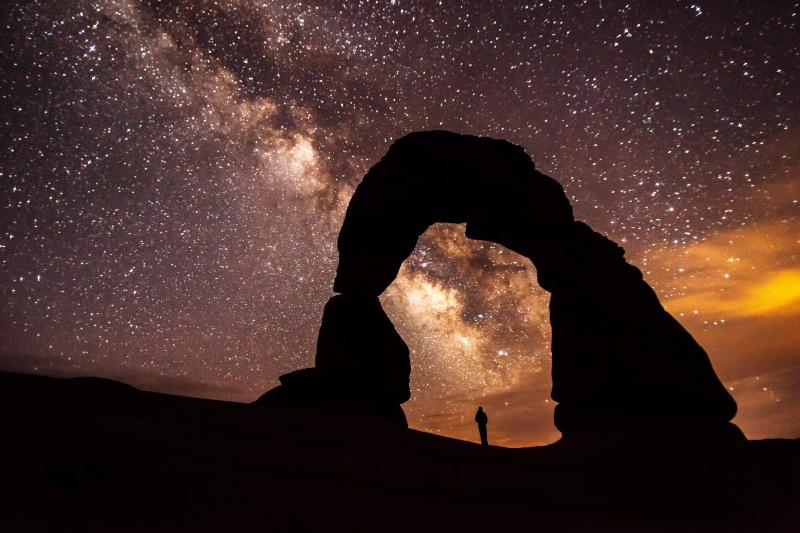
\includegraphics[height=4in]{Figures/delicate_arch.jpg}}

\end{frame}

\end{document}
